% Preserve the template's Times fonts with pdfLaTeX and XeTeX/Tectonic.
\RequirePackage[T1]{fontenc}
\documentclass[letterpaper,10pt,conference]{ieeeconf}

\IEEEoverridecommandlockouts
\overrideIEEEmargins

\usepackage{amsmath,amssymb}
\usepackage{booktabs}
\usepackage{capt-of}
\usepackage{cite}
\usepackage{graphicx}
\usepackage{url}

\title{ClothDojo: A Benchmark and Scalable Data Pipeline for Garment
Flattening and Folding}

% Keep the review draft anonymous until the target venue is fixed.
\author{Anonymous Authors}

\IEEEaftertitletext{%
  \vspace{-1.0em}
  \begin{center}
    \begin{minipage}{\textwidth}
      \centering
      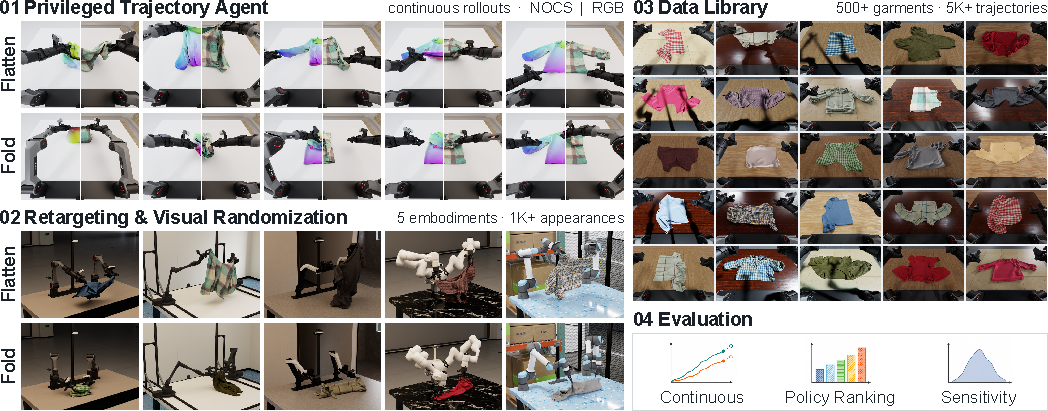
\includegraphics[width=\linewidth]{figures/clothdojo-framework.pdf}
      \captionof{figure}{\textbf{ClothDojo connects data generation, data
      expansion, and closed-loop evaluation.} (01) A trajectory
      agent with privileged visual observations generates flattening and
      folding trajectories, shown with normalized object coordinate space
      (NOCS) and standard RGB appearances side by side. (02) Retargeting across
      robot embodiments and visual randomization expand the data. (03) Garment
      assets and manipulation trajectories form a data library. (04)
      Evaluation uses continuous metrics, policy ranking, and sensitivity
      analysis.}
      \label{fig:framework}
    \end{minipage}
  \end{center}
  \vspace{0.4em}
}

\begin{document}

\maketitle
\thispagestyle{empty}
\pagestyle{empty}

\begin{abstract}
Flattening and then folding a severely crumpled garment is a challenging test
of generalist visuomotor policies. Real-robot experiments are costly and
difficult to reproduce, while existing simulation studies provide limited
evaluation across diverse garments and complex initial states. We present
ClothDojo, a simulation benchmark and data pipeline for garment flattening and
folding. ClothDojo supports real-time bimanual interaction and closed-loop
policy evaluation on a shared test set spanning diverse garments and complex
initial states. To reduce reliance on hand-designed manipulation rules for data
collection, we decouple physical trajectory generation from appearance
randomization. A trajectory agent uses privileged visual information and is
initialized from human demonstrations. It is continually improved through
autonomous rollouts and human interventions, then generates successful
trajectories on new garments and initial states. These trajectories are
re-rendered with randomized appearances to provide diverse RGB observations for
downstream policy training. We use ClothDojo to study how additional
manipulation experience and visual diversity each affect generalization, and to
assess the roles of memory and real-time control in handling occlusion and
dynamic manipulation.
\end{abstract}

\begin{figure*}[t]
  \centering
  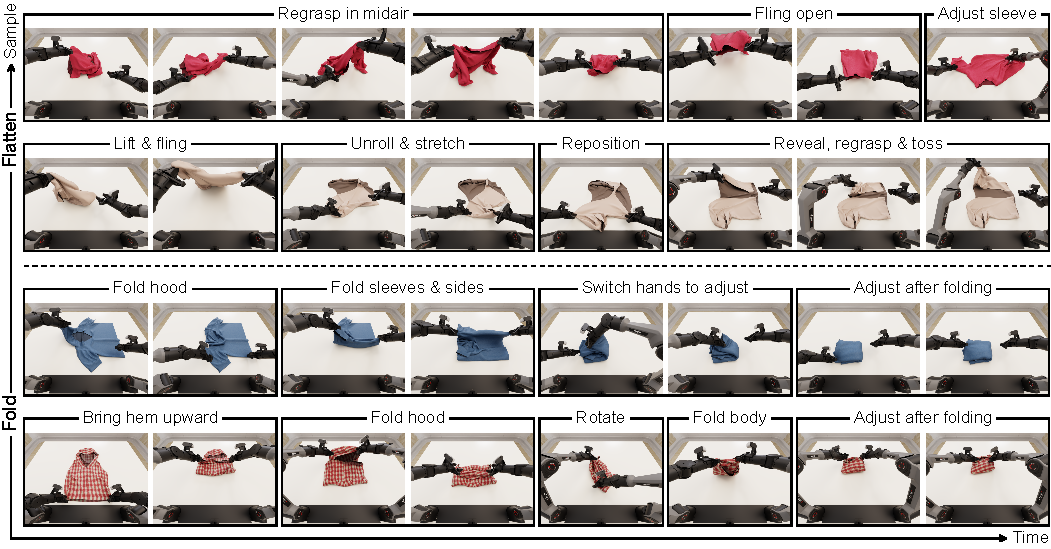
\includegraphics[width=\textwidth]{figures/clothdojo-manipulation-sequences.pdf}
  \caption{\textbf{Autonomous policies generate long-horizon behaviors with
  varied action transitions and adjustments during execution.} Flattening
  trajectories combine midair regrasping, dynamic unfolding, and local
  adjustments; folding includes hand switching, garment rotation, and
  post-fold adjustments. Each row shows keyframes from an independent rollout,
  ordered from left to right with nonuniform time intervals. Box labels
  describe observed behaviors; the images are re-rendered from recorded
  simulation states.}
  \label{fig:folding-trajectories}
\end{figure*}

\section{Introduction}
\label{sec:introduction}

Generalist visuomotor policies should reliably complete tasks across unseen
objects and complex states, adjusting subsequent actions based on observed
outcomes. Garment flattening and folding are well suited for evaluating these
capabilities. Garments vary widely in structure and appearance. Severe
crumpling causes self-occlusion, making the current configuration difficult to
infer. Completing the task requires both dynamic actions, such as flinging, and
precise local adjustments during flattening and folding.

Garment manipulation has been used to evaluate generalist policies on real
robots, but large-scale, reproducible comparisons remain difficult: data
collection, scene setup, and task resets require sustained human effort, and
garment initial configurations are difficult to reproduce precisely.
Simulation provides controlled experimental conditions and supports both data
reuse and scalable evaluation. However, existing simulation benchmarks provide
limited coverage of diverse garments and complex initial states, and their
datasets contain few successful trajectories that complete both flattening and
folding.

We present ClothDojo, a platform for data generation and policy evaluation in
garment flattening and folding. ClothDojo supports real-time dynamic
interaction between multiple bimanual robot embodiments and diverse garments.
Starting from severely crumpled states, closed-loop policies use flinging and
local adjustments to flatten garments, then continue to fold them. Unified
metrics measure task progress and final outcomes.

To scale the successful trajectories needed for downstream policy training,
ClothDojo decouples physical trajectory generation from appearance
randomization. A trajectory agent uses privileged visual information and is
initialized from human demonstrations. It is continually improved through
autonomous rollouts and human interventions. The resulting agent generates
successful closed-loop trajectories on new garments and initial states. We
then re-render these trajectories with randomized appearances while preserving
the underlying behavior, producing diverse RGB observations.

We use ClothDojo to study what enables generalist visuomotor policies to
complete this task. Paired experiments separate the effects of new physical
trajectories and appearance re-renderings, while controlled policy comparisons
test the roles of observation history, memory, and real-time control. We
evaluate all policies in closed loop on held-out initial states across seen and
unseen garments, reporting both stage-wise and end-to-end performance.

\begin{figure*}[t]
  \centering
  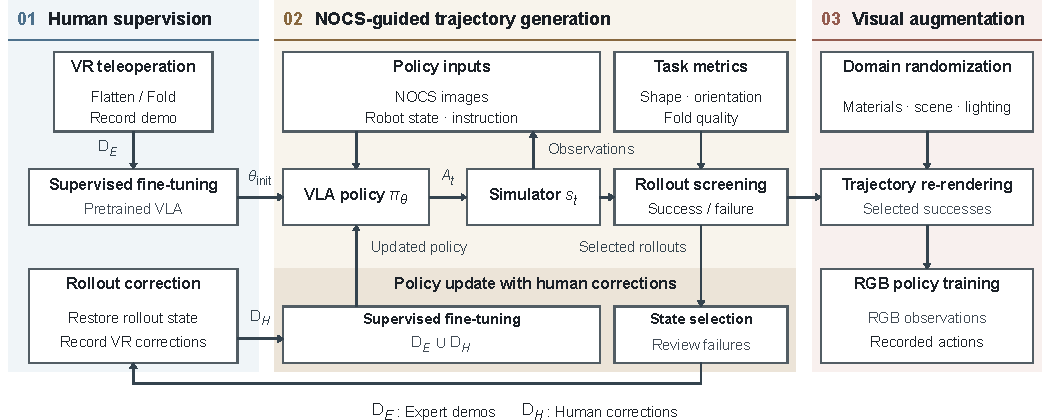
\includegraphics[width=\textwidth]{figures/clothdojo-method-framework.pdf}
  \caption[Overview of the NOCS-guided data engine.]{\textbf{Overview of the NOCS-guided data-generation pipeline.}
Expert demonstrations $\mathcal D_E$ initialize a trajectory agent. For
failures encountered during autonomous execution, an operator restores a
selected state and provides a correction $\mathcal D_H$. The two sources of
human data update the agent, while successful rollouts are re-rendered under
randomized appearances to train an RGB policy.
}
  \label{fig:method-framework}
\end{figure*}
\section{Related Work}
\label{sec:related-work}

\subsection{Garment manipulation}

Garment manipulation has commonly been made tractable by reducing control to
task-specific primitives, such as selecting grasp points followed by a fixed
pick--place or fling motion. These methods encode useful geometric and control
knowledge and can solve well-defined garment tasks efficiently. At the same
time, the primitive determines much of the behavior before learning begins. It
therefore provides limited evidence about whether a generalist policy can infer
garment state, produce continuous robot motion, and recover from its own
mistakes. ClothDojo retains the ordinary robot action interface so that these
abilities remain part of the evaluated problem.

\subsection{Deformable simulation and benchmarks}

Simulation environments, simulation benchmarks, and policy benchmarks answer
different questions. An environment determines what can be simulated; a
fidelity benchmark measures how well simulated cloth matches physical cloth;
a policy benchmark measures what an agent can accomplish under a fixed task
distribution. GarmentLab and RGBench primarily strengthen the first two
layers. SimWeaver additionally connects simulation to policy training and is
therefore the closest setting to ClothDojo. ClothDojo concentrates on the third
layer: severe garment flattening with continuous actions, scalable successful
data, and closed-loop evaluation across garment variation.

\subsection{Data generation for generalist robot policies}

Privileged supervision separates the difficulty of producing useful training
behavior from the difficulty of the final visual task. NOCS supplies stable
cross-asset geometric cues to the trajectory agent while preserving the VLA's
image-to-action structure. Once a successful physical trajectory exists, its
observations can be rendered without those cues. Thus the downstream policy
still acts from ordinary images and never accesses particle state; privilege is
used to manufacture data, not to simplify the evaluated policy.

\section{Method}
\label{sec:method}

ClothDojo separates physical trajectory generation from visual data expansion
(Fig.~\ref{fig:method-framework}). We first train NOCS-conditioned trajectory
agents from human demonstrations and corrections, then deploy them on unseen
garments and initial states. We automatically filter the resulting rollouts
using task metrics and re-render the successful ones under different appearances to train RGB
policies. One successful physical rollout can thus yield multiple visual
versions without regenerating its actions.

\subsection{Interaction environment and tasks}

ClothDojo combines MuJoCo robot dynamics~\cite{todorov2012mujoco} with Style3D
cloth simulation in Newton~\cite{newton} to support continuous bimanual
control. Virtual reality (VR) teleoperation and policy execution use the same
physics, so human
demonstrations, corrections, and autonomous rollouts share the same
robot--cloth interaction. Fig.~\ref{fig:folding-trajectories} shows
autonomous trajectories in which the agents repeatedly grasp, coordinate both
arms, and adjust their actions as the cloth state changes.

We convert more than 10,000 garments from the large-scale parametric
GarmentCodeData dataset~\cite{GarmentCodeData} into simulation assets and
select 500 structurally diverse garments for our experiments. As shown in
Fig.~\ref{fig:garment-assets}, this set spans large variations in garment
length, body width, sleeve length, and sleeve width, and includes sleeveless,
hooded, low-cut, open-back, asymmetric, and unconventional designs.

\begin{figure}[t]
  \centering
  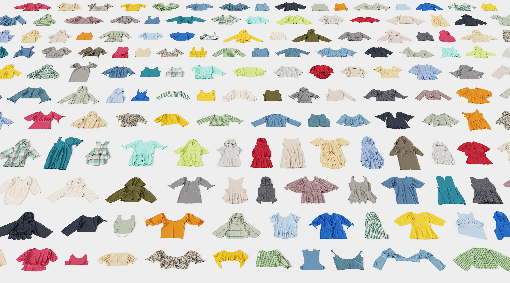
\includegraphics[width=\linewidth]{figures/clothdojo-garment-assets.pdf}
  \caption{\textbf{The experimental garment set spans diverse geometries.}
  The figure shows most of the 500 assets, covering different garment lengths,
  widths, sleeve types, necklines, and asymmetric cuts. All garments are
  naturally settled and shown at their relative physical sizes.}
  \label{fig:garment-assets}
\end{figure}

\textbf{Flattening} starts from a crumpled state produced by randomly hanging,
releasing, and settling a garment. The goal is a naturally flat, face-up
configuration. All four cardinal orientations on the table are accepted, and its
position within the tabletop is unconstrained. \textbf{Folding} starts from a
successful final state of the preceding flattening task. The goal is a compact,
flat rectangular bundle with little protruding material. We prescribe no
aspect ratio, crease pattern, or action order. Initial states for both tasks
are saved in advance so that policies can run from identical states; the
quantitative success criteria are given in Sec.~\ref{sec:success-criteria}.

\subsection{NOCS-conditioned trajectory agents}

We provide a surface-position reference that remains consistent as the cloth
deforms by encoding normalized object coordinate space
(NOCS)~\cite{wang2019nocs} as the garment texture. Let $v_i$ denote a vertex
of the canonical mesh, with component-wise bounds $v_{\min}$ and $v_{\max}$.
Its normalized coordinate is
\begin{equation}
  u_i=\frac{v_i-v_{\min}}{v_{\max}-v_{\min}},
  \label{eq:nocs-color}
\end{equation}
whose three components form the RGB channels. Each color is assigned in the
canonical configuration and remains attached to the corresponding vertex as
the garment deforms. Similar relative positions across garments therefore
receive similar colors. This exposes canonical surface-position cues through
the model's existing image interface. The agent still observes only visible
surfaces, and matching colors do not imply exact semantic correspondence
across garments.

We use the pretrained $\pi_{0.5}$ model~\cite{pi05} as the base and separately
fine-tune trajectory agents for flattening and folding. Each agent receives
NOCS images through the model's original visual interface, together with the
robot state and task instruction, and predicts joint targets and gripper
commands for both arms. During execution, the agent applies only a prefix of
each predicted action sequence and then replans from the latest observation,
producing a closed-loop trajectory.

\subsection{Learning from demonstrations and corrections}
\label{sec:experience-corrections}

We collect separate flattening and folding demonstrations through VR
teleoperation. To collect a folding demonstration, we restore the final state
of its corresponding flattening demonstration and continue from that state.
The tasks are recorded separately and used to fine-tune their respective
agents with the base model's action-prediction objective. Sec.~\ref{sec:trajectory-agent-eval}
reports the garment coverage and number of demonstrations.

To cover states induced by the agents themselves, we use DAgger-like iterative
data aggregation~\cite{DAgger}. Each agent first rolls out autonomously on
different garments and initial states. For an execution that requires
correction, an operator selects an intervention point, restores that simulation
state, and continues the task through VR, producing a correction trajectory
$\mathcal D_H$. We then combine these corrections with the original
demonstrations $\mathcal D_E$ and update the agent using the same supervised
objective. All supervised actions are provided by humans; at this stage,
autonomous rollouts supply the starting states for correction.

To add training examples with exchanged arm roles, we apply bilateral
morphological symmetry augmentation~\cite{GR-RL} to every human trajectory.
At each frame, we reflect the garment state and transform the robot states and
actions while exchanging the two arms and grippers. We then re-render NOCS
observations by replaying the transformed states. Each human trajectory yields
one mirrored sample, which is not counted as an additional human demonstration.

\subsection{RGB data from successful trajectories}

After training, we freeze the trajectory agents and roll them out
autonomously on unseen garments and initial states. The task criteria in
Sec.~\ref{sec:success-criteria} automatically filter the results, retaining only
successful trajectories.

For each successful trajectory, we sample from 34 base garment materials with
39 color variants, 17 table materials, 12 floor materials, and eight
background scenes. Light position, intensity, and color temperature are drawn
from continuous ranges. Each appearance remains fixed within a trajectory. We
replay the saved states to render RGB observations while preserving the robot
and garment motion, robot states, and action targets. The resulting data train
downstream policies that receive RGB observations, robot states, and task
instructions without NOCS. A physical trajectory may produce multiple visual
versions, but we count it as one manipulation experience. The appearance
subsets used for training and evaluation are specified in the experimental
setup.

\section{Experiments}
\label{sec:experiments}

\subsection{Benchmark protocol and baselines}

A useful benchmark must be reproducible, difficult enough to separate methods,
and rich enough to explain the separation. Representative policies therefore
operate on the same garments and initial states under the same closed-loop
budget. Success measures task completion, while distance and difficulty strata
show whether two policies fail in the same way.

\subsection{Does NOCS produce a better trajectory agent?}

NOCS is justified only if it improves the ability to produce successful
physical trajectories, rather than merely making training loss smaller. NOCS
and ordinary-appearance agents therefore share demonstrations, architecture,
optimization, and evaluation cases. Their success and distance across data
scales and garments measure the value of the privileged representation.

\subsection{What does generated data add?}

Generated data can add either new behavior or new appearance. Re-rendering a
fixed trajectory tests visual diversity alone; generating new trajectories
tests state--action diversity; combining both tests their interaction. Varying
garment breadth separately from trajectories per garment then reveals whether
downstream learning benefits from more structural coverage or denser practice
on familiar structures.

\subsection{Where do current policies fail?}

Aggregate success mixes several causes of failure. Conditioning results on
initial distance and garment morphology exposes geometric difficulty. Holding
the physical case fixed while changing texture, background, or lighting exposes
visual sensitivity. Changing validated physical parameters exposes dynamics
sensitivity. Together these views turn the task into a diagnostic benchmark
rather than a single leaderboard number.

\subsection{Do memory and action models help?}

Flattening creates reasons for temporal reasoning that are absent from a
single-frame task. Earlier views can reveal garment identity before it becomes
occluded, and the result of a failed dynamic action indicates how the next
action should change. History, explicit memory, action chunking, RTC, and
world-action models represent different ways to use this information. Their
value is determined by where they improve recovery and difficult cases, not by
their average score alone.

\subsection{Dynamics and real-world transfer}

Dynamic actions couple cloth properties with robot execution. Changes in
friction, stiffness, damping, tracking bandwidth, or action latency can alter
the result of an otherwise identical command. Robustness experiments therefore
test whether a policy observes and corrects physical outcomes instead of
replaying a fixed motion. Real-data experiments hold human data fixed so that
any gain can be attributed to the additional simulated trajectories.

\section{Limitations and Conclusion}
\label{sec:conclusion}

ClothDojo treats severe garment flattening as both a data problem and an
evaluation problem. The environment makes continuous dynamic interaction
available, the privileged trajectory agent makes successful behavior scalable,
and the benchmark turns garment, state, appearance, and dynamics variation into
controlled evidence about generalist policies. Its conclusions remain bounded
by upper-body garment coverage, simulation fidelity, trajectory-agent coverage,
and the extent of real-world validation.


\bibliographystyle{IEEEtran}
\bibliography{references}

\end{document}
